\subsection{Business Rules} \label{subsec:BusinessRules}

% TODO: Parameterize business rules

\begin{itemize}
    \item All of the book's words are sorted alphabetically without regard to capitalization (for example, ``hello'' occurs after ``Hear'' and before ``HELP'')
    \item The word occurs \textit{occurrences} times in the book
%    \item If $occurrences$ is an even number then the response word is the word is $occurrences$ places \textbf{after} the challenge word in the alphabetized list;
%    if the challenge word is less than $occurrences$ places from the start of the list then the response word is the first word in the list
%    \item If $occurrences$ is an odd number then the response word is the word $occurrences$ places \textbf{before} the challenge word in the alphabetized list;
%    if the challenge word is less than $occurrences$ places from the end of the list then the response word is the last word in the list
\end{itemize}

As a simple example, look at the \textit{Food} file.
After sorting and counting, we have:

\begin{center}
    \begin{tabular}{cc}
        \textit{word} & \textit{occurrences} \\ \hline
        apple       & 7 \\
        banana      & 4 \\
        carrot      & 15 \\
        date        & 3 \\
        eggplant    & 2 \\
        fig         & 6 \\
        granola     & 9 \\
        horseradish & 9 \\
        ice         & 6 \\
        jelly       & 3 \\
        kale        & 1 \\
        lemon       & 2 \\
        mango       & 8 \\
        naan        & 7 \\
        orange      & 5 \\
        pineapple   & 1 \\
        quinoa      & 11 \\
        raisin      & 4 \\
        spaghetti   & 10 \\
        tomato      & 12 \\
    \end{tabular}
\end{center}

You break the problem down into three sub-problems:

\begin{enumerate}
    \item Designing the Data Structure and Its Algorithms
    \item Alphabetizing Words
    \item Inserting Words
%    \item Responding to a Challenge
\end{enumerate}

\subsubsection*{The Books}

Four small ``books'' are included with the starter code:

\begin{itemize}
    \item ``Animals'' (sorted, 7 words)
    \item ``Plants'' (unsorted, 7 words)
    \item ``Cars'' (sorted, 74 words)
    \item ``Food'' (unsorted, 125 words)
\end{itemize}

Two real books have also been reduced to one word per line:\footnote{The text for these books was obtained from \href{https://www.gutenberg.org/}{Project Gutenberg}.
In accordance with Paragraph~1.C of the \href{https://www.gutenberg.org/policy/license}{Project Gutenberg License}, all references to Project Gutenberg have been removed from the ``derived works'' that we are distributing.
    (Removing the references to Project Gutenberg was also necessary to ensure that \textit{only} the words from the books are included in the list.)}

\begin{itemize}
    \item Mary Shelly's \textit{Frankenstein; Or, The Modern Prometheus} (filename ``Frankenstein'') \url{https://www.gutenberg.org/ebooks/84} (sorted, 74,363 words)
    \item Arthur Conan Doyle's \textit{The Lost World} (filename ``TheLostWorld'')
    \url{https://www.gutenberg.org/ebooks/139} (unsorted, 77,268 words)
\end{itemize}

The very small files of 7 words can be useful for debugging, and the moderate-sized files of 74--125 words should give you confidence in the correctness of your solution.
The real books of more than 74,000 words will be useful to reveal whether you have any memory leaks in your code.
The files marked as \textit{sorted} have all of their words already in alphabetically sorted order, ignoring capitalization;
the files marked as \textit{unsorted} do not have their words sorted (the words in ``Plants'' and ``Food'' are in a randomly-selected order;
the words in ``TheLostWorld'' appear in the order that they appear in the original \textit{The Lost World}).

Each book file, ``\textit{file}'', has a corresponding ``\textit{file}-table.md'' that contains a Markdown-formatted table of the words and the number of occurrences for each word.
You may use these files to confirm the correctness of your solution.

Throughout the assignment, we note that if building the list takes more than a few seconds, there is a bug in your code;
You should be able to build a list for \textit{Frankenstein} or \textit{The Lost World} in under a second.
Your code may take longer, but it should not take much longer.

\colorbox{yellow}{Some of the tests in \textit{sorted-test.c} will timeout after ten seconds to stop runaway code.} \\
\colorbox{yellow}{To disable this timeout (such as when debugging with breakpoints), compile the code with} \\
\colorbox{yellow}{\texttt{touch sorted-list.c; make OPTION="-DNOTIMEOUT"}} \\
(to re-enable the timeout, use \texttt{touch sorted-test.c; make})

You will earn most of the credit for this lab if your code works for pre-sorted files of up to 200 words.
The remaining credit is for making your code work with unsorted files and, when using files of up to 80,000 words, your code can generate a list and find a word in fewer than 20 seconds.

\vspace{1cm}

H.Awk provides you with the code he worked on.
It turns out that while he finished implemented the array-backed list, he didn't finish the sorting algorithm.
You decide to warm up by finishing the app and then circling back to the linked list.

\subsection{Word Entries}

The \lstinline{word_entry_t} type is defined in \textit{word\_entry.h}:

\lstinputlisting[linerange=28-31, firstnumber=28]{../starter-code/word_entry.h}

You see that there are also a handful of function prototypes in \textit{word\_entry.h} that would nicely encapsulate this datatype.

\subsubsection{Creating and Destroying Word Entries}

The \function{create_word_entry()} function allocates space for a \lstinline{word_entry_t}, and the \function{delete_word_entry()} function releases that memory.
The \function{create_word_entry()} function, however, does not yet initialize the word entry.

\begin{description}
    \checkoffitem{In \function{create_word_entry()}'s \lstinline{else} block, copy \lstinline{word} into \lstinline{word_entry}'s \lstinline{word} field.}
    \checkoffitem{In \function{create_word_entry()}'s \lstinline{else} block, set \lstinline{word_entry}'s \lstinline{occurrences} field to 0.}
\end{description}

When you copy the word, you must actually copy the word and not merely copy the pointer, for two reasons.
The first reason, from a program design perspective, is that you don't know whether the caller might later put a different word in the array that the \lstinline{word} parameter is in, or the caller might even deallocate that array's memory.
The second reason, from a memory perspective, is that an array embedded in a \lstinline{struct} (such as \lstinline{word_entry_t}'s \lstinline{word} field) is effectively a constant pointer and cannot be re-assigned.

You do not need to make any changes to \function{delete_word_entry()}.

\subsubsection{Accessors and Mutators \\ \footnotesize{\textit{aka}, Getters and Setters}}

We want to control the possible changes that other code might make to a word entry.
Indeed, the only reasonable change would be to increase the number of times that the word is found in a book, whenever we encounter that word again.
Similarly, we want to make sure that data that our ``getter'' functions cannot be used by the caller to make changes to the structure's data.
The \function{get_count()} function returns a value, so there's no hazard there.
The \function{get_word()} function returns a pointer to a constant -- while it \textit{is} possible to discard a \lstinline{const} qualifier, doing so will result in a warning that it will result in undefined behavior.
(The array that the pointer points to isn't actually constant, but the caller is obligated to act as though it is.)

\begin{description}
    \checkoffitem{In \function{increment_count()}, increase the word entry's number of occurrences by one.}
    \checkoffitem{In \function{get_count()}, return the number of occurrences.}
    \checkoffitem{In \function{get_word()}, return a pointer to the word entry's word. (Do \textit{not} make a copy of the word.)}
\end{description}

When returning the word entry's word, simply returning the pointer is sufficient -- and desirable.
It is sufficient because the caller is obligated to treat it as a constant.
The alternative, making a copy, is not desirable because the function doesn't expect the caller to provide a destination, which means that the function would have to allocate memory for the destination;
the caller would be unable to later free this memory without discarding the \lstinline{const} qualifier.

\paragraph{Testing Your Changes}

You can build an executable that uses H.Awk's array-backed list with the command \\
\verb+make arraylist+ \\
or, if you want to limit each \function{malloc()} call to no more than 32KB, then use the command \\
\verb+make arraylist "OPTION=-DHOBBLE"+

\begin{description}
    \checkoffitem{Build and run the executable.         \\
        \texttt{0) Quit                                 \\
                1) Test word\_entry                     \\
                2) Test list                            \\
                3) Test alphabetical functions          \\
                4) Test insert\_word (empty list)       \\
                5) Test insert\_word (singleton list)   \\
                6) Test insert\_word (populated list)   \\
                7) Create and print book list           \\
                Select the task you wish to check:}}
    \checkoffitem{Select task 1, ``Test word\_entry''.  \\
        \texttt{0) Return to main menu                  \\
                1) create\_word\_entry()                \\
                2) delete\_word\_entry()                \\
                3) increment\_count()                   \\
                4) get\_count()                         \\
                5) get\_word()                          \\
                Select the function you wish to check:}}
    \checkoffitem{Select function 1, ``create\_word\_entry()'', and enter a word when prompted.}
\end{description}

The word entry will be displayed.
For example, if your word was ``foo'' then the output will be: \\
\texttt{Created --           0 : foo}

\begin{description}
    \checkoffitem{Use fuctions 3 (``increment\_count()''), 4 (``get\_count()''), and 5 (``get\_word()'') to test your code.}
    \checkoffitem{Continue to test until you discover a bug or are satisfied that your implementations are correct.}
    \checkoffitem{When you have finished, use function 2 (``delete\_word\_entry()'') to release the word entry's memory, then select 0 to return to the main menu, and then select 0 to exit the program.}
    \begin{itemize}
        \item Note: whenever you return to the main menu, any existing list will be deleted.
            No memory references survive when moving between one main-menu-option and another.
    \end{itemize}
\end{description}



\subsection{Alphabetical Functions}

\subsubsection{Making a Lowercase Copy of a Word}

Because the book's words should be insensitive to capitalization, we will store the words with all of their letters in lowercase.
In \textit{challenge-response.c}, there is a \function{word_to_lowercase()} function to do just that.

\begin{description}
    \checkoffitem{Implement the \function{word_to_lowercase()} function.}
\end{description}

Unlike keyboardlab, you can use the \function{tolower()} function\footnote{\url{https://en.cppreference.com/w/c/string/byte/tolower}} from \texttt{ctype.h}.

\subsubsection{Comparing Words}

Because the book's words need to be sorted, we need to be able to compare words.
In \textit{challenge-response.c}, there are three functions to do that:
\begin{description}
    \item[words\_are\_equal()] which returns \lstinline{true} if and only if the two words are indistinguishable
    \item[word1\_is\_earlier\_than\_word2()] which returns \lstinline{true} if and only if the first word precedes the second word in an alphabetically-sorted list
    \item[word1\_is\_later\_than\_word2()] which returns \lstinline{true} if and only if the first word follows the second word in an alphabetically-sorted list
\end{description}

\begin{description}
    \checkoffitem{Implement the \function{words_are_equal()} function.}
    \checkoffitem{Implement the \function{word1_is_earlier_than_word2()} function.}
    \checkoffitem{Implement the \function{word1_is_later_than_word2()} function.}
\end{description}

We recommend that you use the \function{strncmp()} function\footnote{\url{https://en.cppreference.com/w/c/string/byte/strncmp}} from \texttt{string.h}.

\paragraph{Testing Your Changes}

You can build an executable that uses H.Awk's array-backed list with the command \\
\verb+make arraylist+ \\
or, if you want to limit each \function{malloc()} call to no more than 32KB, then use the command \\
\verb+make arraylist "OPTION=-DHOBBLE"+

\begin{description}
    \checkoffitem{Build and run the executable.         \\
        \texttt{0) Quit                                 \\
                1) Test word\_entry                     \\
                2) Test list                            \\
                3) Test alphabetical functions          \\
                4) Test insert\_word (empty list)       \\
                5) Test insert\_word (singleton list)   \\
                6) Test insert\_word (populated list)   \\
                7) Create and print book list           \\
                Select the task you wish to check:}}
    \checkoffitem{Select task 3, ``Test alphabetical functions'', and enter words when prompted.}
\end{description}

Each word will be displayed in its lowercase form, and the results of the three comparison functions will be shown.

\begin{description}
    \checkoffitem{Continue to test until you discover a bug or are satisfied that your implementations are correct.}
    \checkoffitem{When you have finished, select 0 to exit the program.}
\end{description}


\subsection{Preparing to Work with Lists}

It is entirely probable that H.Awk, left to his own devices, would simply have used an array instead of making the effort to create an array-backed list with a well-defined abstract model.
Fortunately, someone pulled his strings, and you have available to you an abstract model of a list that can be realized by any number of implementations.

Like \lstinline{word_entry_t}, the \lstinline{list_t} and the \lstinline{iterator_t} datatypes have functions to encapsulate them.
In the case of \lstinline{list_t} and \lstinline{iterator_t}, however, this encapsulation is essential because the code in \textit{sorted\_word\_entries.c} has access to the type declaration but not the type definition.

\begin{description}
    \checkoffitem{Review the datatypes and functions declared in \textit{list.h}.}
\end{description}

A list is abstractly modeled as having a sequence of word entries and an iterator that points to the ``current'' word entry.
The iterator can point to anywhere between the first word entry and the last word entry.

\textcolor{red}{
A good rule of thumb is that if the previous operation returned the iterator, then the iterator is valid;
if the previous operation returned the list, then the iterator is invalid and should not be used.
Attempting to access non-existent word entries beyond the bounds of the list will also invalidate the iterator.
}

\begin{itemize}
    \item The \function{get_iterator()} function sets the iterator to the first word entry, and the \function{iterate_next()} and \function{iterate_previous()} functions cause the iterator to advance and retreat
    \item The \function{has_next()} and \function{has_previous()} functions report whether there are additional word entries in the indicated direction
    \item The \function{get_word_entry()} function retrieves the word entry that the iterator points to, and the \function{get_next_word_entry()} and \function{get_previous_word_entry()} functions retrieve the word entry in the indicated direction
    \item The \function{prepend()} and \function{append()} functions place a word entry at the beginning or end of the list, respectively, setting the iterator to the new word entry
    \item The \function{insert()} function places a new word entry at the iterator's location, and the function{delete()} function removes the word entry at the iterator's location -- both of these functions invalidate the iterator
    \item The \function{swap_next()} and \function{swap_previous()} functions can be used to move a word entry forward and backward
    \item The \function{merge_next()} and \function{merge_previous()} functions can be used to combine a word entry with its neighbor
\end{itemize}

\begin{description}
    \checkoffitem{Review the \function{test_list()} function in \textit{list-test.c} to see uses of the \lstinline{list_t} and \lstinline{iterator_t} functions.}
    \checkoffitem{Run the arraylist executable, selecting task 2 (``Test list'') to observe the behavior of the \lstinline{list_t} and \lstinline{iterator_t} functions.}
\end{description}


\subsection{Inserting Words}

The \function{build_list()} function in \textit{sorted\_word\_entries.c} reads words from a ``book'' and sends them to \function{insert_word()}.
You do not need to implement \function{build_list()}.

The \function{insert_word()} function in \textit{sorted\_word\_entries.c} finds the correct place in the list for a lowercase copy of the word.
If the word is already in the list, then it increments the word's count;
otherwise, it inserts the word into the list.
You will implement \function{insert_word()}.

\subsubsection{Limited Implementation}

The simplest implementation of \function{insert_word()} is to assume that the words in the book are already sorted -- as they are for ``Animals'', ``Cars'', and ``Frankenstein''.
In this case, you know that if the word is already in the list then it is the last word in the list,
and if the word is not already in the list then it belongs at the end of the list.

You will receive half of the credit for \function{insert_word()} if it works on pre-sorted books.
If you choose to use this implementation:
\begin{description}
    \checkoffitem{Implement \function{insert_word()} for pre-sorted books}
    \checkoffitem{Test this implementation and move on to implementing a linked list}
    \checkoffitem{Return to this sub-problem later to attempt a more-general implementation}
\end{description}

Otherwise, implement Insertion Sort\dots

\subsubsection{Insertion Sort}

While you probably learned about sorting in \cstwo, you may not have learned about \textit{Insertion Sort}.
If you did learn about Insertion Sort, you probably learned to use it to sort an array or list in-place, and that it's a $\mathcal{O}(n^2)$ algorithm that is less efficient than $\mathcal{O}(n \log n)$ sorting algorithms such as Merge Sort and Quick Sort.
Insertion Sort is often taught as a way to sort an array in-place,
but a variation of Insertion Sort has a particular advantage in that it can be applied \textit{as the list is built}, making for a much simpler and less error-prone implementation than a different sort that requires the list to already be built.

Your Insertion Sort algorithm will read an input and then traverse a sorted list to find the proper location in the sorted list for the input.
The input is then inserted into the list at that location, preserving the property that the list is sorted.

\begin{description}
    \checkoffitem{Implement \function{insert_word()} such that:}
    \begin{itemize}
            \item The word is placed at the end of the list
            \item If the word is not in its proper location, then it is moved to is proper location
            \item Once in its proper location, if there is another word entry with the same word, then the two word entries are combined
        \end{itemize}
\end{description}

\paragraph{Testing Your Changes}

If you were to apply category-partition testing, you might arrive at these categories and partitions:

\begin{center} \begin{tabular}{c|c}
    \textbf{Categories}             & \textbf{Partitions}                   \\ \hline\hline
    Word's position in the list     & only word in the list                 \\
                                    & at the start of the list              \\
                                    & at the end of the list                \\
                                    & somewhere in the middle of the list   \\ \hline
    The list's initial length       & no words                              \\
                                    & one word                              \\
                                    & more than one word                    \\ \hline
    Word is already in the list?    & yes                                   \\
                                    & no                                    \\ \hline
    Word is already lowercase?      & yes                                   \\
                                    & no
\end{tabular}\end{center}

\begin{description}
    \checkoffitem{Build and run the executable.         \\
        \texttt{0) Quit                                 \\
                1) Test word\_entry                     \\
                2) Test list                            \\
                3) Test alphabetical functions          \\
                4) Test insert\_word (empty list)       \\
                5) Test insert\_word (singleton list)   \\
                6) Test insert\_word (populated list)   \\
                7) Create and print book list           \\
                Select the task you wish to check:}}
\end{description}

You can test ``only word in the list''/``word is not already in the list'' with task 4.
You can test most of the other combinations with tasks 5 \& 6.
When you select these options, an initial sorted list (empty or pre-populated, as appropriate) will be created and printed, and you will be prompted to enter a word.
After you have entered a word, \function{insert_word()} will be called, and the resulting sorted list (with a new word with 1 occurrence, or with an existing word's occurrences increased by 1) will be printed.

\begin{description}
    \checkoffitem{Test \function{insert_word()} until you discover a bug or are satisfied that your implementation is correct.}
\end{description}


\subsection{Testing the System with ``Books''} \label{subsec:TestingChallengeResponse}

When you are satisfied that your word entry, alphabetical, and word insertion functions are correct, test them with book files.
With task 7, you will be prompted for the name of a book file, and then the list will be generated and printed.
You can use the ``\textit{file}-table.md'' files to confirm the correctness of the results.

\textcolor{red}{If your program requires more than a few seconds to build a list, then there is a bug in your code.}

\begin{description}
    \checkoffitem{Test building a list until you discover a bug or are satisfied that your implementations are correct.}
%    \checkoffitem{Test challenge/responses until you discover a bug or are satisfied that your implementations are correct.}
    \checkoffitem{When you have finished, select 0 to exit the program.}
\end{description}

As a reminder, the book files are:

\begin{itemize}
    \item ``Animals'' (sorted, 7 words)
    \item ``Plants'' (unsorted, 7 words)
    \item ``Cars'' (sorted, 74 words)
    \item ``Food'' (unsorted, 125 words)
    \item ``Frankenstein'' (sorted, 74,363 words)
    \item ``TheLostWorld'' (unsorted, 77,268 words)
\end{itemize}


\section{Linked List} \label{sec:LinkedList}

\textit{n.b.}: If you need a refresher on linked lists, see Appendix~\ref{sec:linkedLists}.

In \textit{list.h}, we use a forward declaration to make the code in \textit{sorted\_word\_entries.c} aware of the types.

\lstinputlisting[linerange=43-43, firstnumber=43]{../starter-code/list.h}
\lstinputlisting[linerange=58-58, firstnumber=58]{../starter-code/list.h}

When you built the \textit{arraylist} executable earlier, the \textit{array\_list.h} file provided type definitions for the code in \textit{array\_list.c} to use.
Similarly, when you build the \textit{linkedlist} executable, the \textit{linked\_list.h} file provides type definitions for the code in \textit{linked\_list.c} to use.

\lstinputlisting[linerange=58-62, firstnumber=58]{../starter-code/linked_list.h}
\lstinputlisting[linerange=71-74, firstnumber=71]{../starter-code/linked_list.h}

The list definition has three pointers, a \lstinline{head} that points to the first node in the list, a \lstinline{tail} that points to the last node in the list, and an \lstinline{iterator}.
The iterator definition has two pointers, a \lstinline{list} that points back to the list structure, and a \lstinline{current_node} that points to the current node, denoting the iterator's position in the list.
\textcolor{red}{
    \begin{itemize}
        \item \lstinline{head} and \lstinline{tail} are \lstinline{NULL} if and only if the list is empty.
        \item \lstinline{current_node} only needs to have a sensible assignment when the iterator is valid.
            When the iterator is invalid, \lstinline{current_node} can be NULL; it can point to a node in the list; it can point to \textit{any} memory location.
    \end{itemize}
}

We define a linked list note conventionally:

\lstinputlisting[linerange=31-31, firstnumber=31]{../starter-code/linked_list.h}
\dots
\lstinputlisting[linerange=41-45, firstnumber=41]{../starter-code/linked_list.h}

(Here the forward declaration is necessary so that \lstinline{node_t} can be used when defining the node structure.)

When writing functions in \textit{sorted\_word\_entries.c}, you had to rely on \lstinline{list_t}'s and \lstinline{iterator_t}'s encapsulation and could not assume any particular list \& iterator definitions.
\textbf{Whenever you are writing a function in \textit{linked\_list.c}, you can treat \lstinline{list_t} and \lstinline{iterator_t} as though they have the linked list definitions.}


\subsection{Building and Testing Your Linked List Implementation} \label{subsec:BuildingLinkedList}

If you use the command \\
\verb+make all+ \\
or \\
\verb+make all "OPTION=-DHOBBLE"+ \\
then you will generate two executables: \textit{arraylist} that has the array-backed list, and \textit{linkedlist} that has the linked list.
If you open two terminal windows, you can run the test code on \textit{arraylist} in one window and run the test suite on \textit{linkedlist} in the other window.
This will allow you to compare the results with your linked list implementation against the expected results provided by the array-backed list (Figure~\ref{fig:SideBySideTesting}).

\begin{figure}
    \centering
    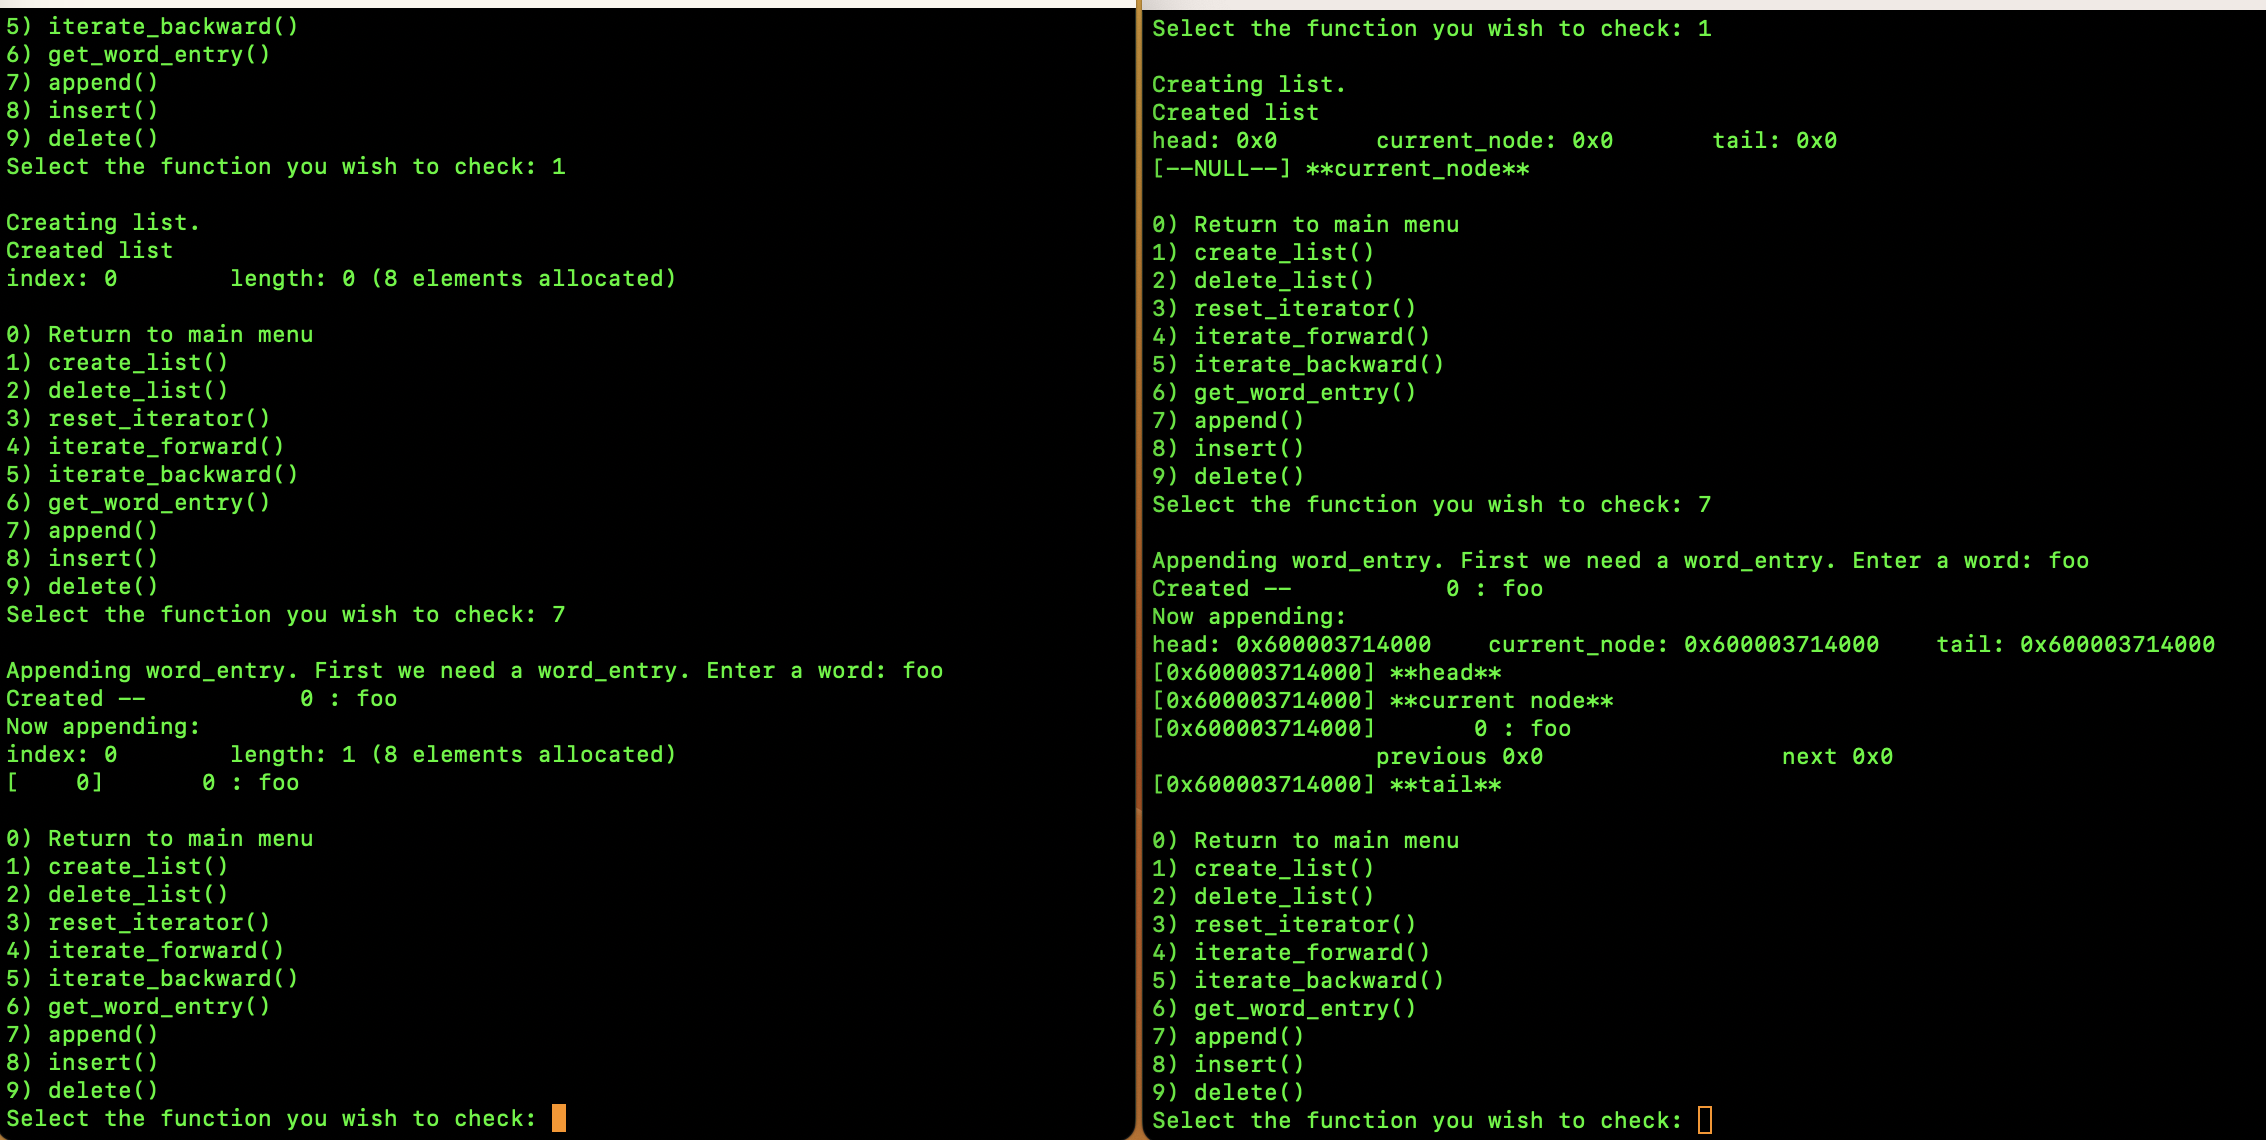
\includegraphics[width=6in]{SideBySideTesting}
    \caption{Testing an array-backed list (left) and a linked list (right) side-by-side.}
    \label{fig:SideBySideTesting}
\end{figure}

To test your linked list implementation, run \textit{linkedlist} (and, optionally, \textit{arraylist} in another terminal window),
and select option 2, ``Test list''


\subsection{Creating a Node, Creating a List}

In \textit{linked\_list.c}:

\begin{description}
    \checkoffitem{Edit \function{create_node()} to initialize all of a new node's fields, as well as those of its iterator.}
    \checkoffitem{Edit \function{create_list()} to initialize all of a new list's fields.
        \begin{itemize}
            \item The list's \lstinline{iterator} field should point to its iterator, and the iterator's \lstinline{list} field should point back to its list (See Section~\ref{subsubsec:listt-as-lined-list}).
        \end{itemize}
    }
    \checkoffitem{Edit \function{get_iterator()} to return the list's iterator.}
    \checkoffitem{Edit \function{get_list()} to return the list's iterator. The current node should be the head of the list.}
    \checkoffitem{Test \function{create_node()} and \function{create_list()} by selecting option 2 (``Test list'') and function 1 (``create\_list()'').}
    \checkoffitem{Test \function{get_iterator()} and \function{get_list()} by selecting functions 3 (``get\_iterator()'') and 4 (``get\_list()'').}
    \checkoffitem{Free the memory by selecting function 2 (``delete\_list()'').
        Exit out of the program by selecting function 0, then option 0.}
\end{description}

It is unlikely that you made any errors that would cause these test to fail,
but it's better to find out now if you did.


\subsection{Prepending and Appending a Node}

The \function{append()} function takes a word entry, makes it the payload of a new node, and places the new node at the start of the linked list.
The new node, of course, becomes the head of the list.
Similarly, the \function{append()} function takes a word entry, makes it the payload of a new node, and places the new node at the end of the linked list.
The new node becomes the tail of the list.
If the list is initially empty, then the new node is both the head and the tail of the list.

\begin{description}
    \checkoffitem{Edit \function{prepend()} to place a word entry at the start of the list. The current node should be the newly-added node.}
    \checkoffitem{Edit \function{append()} to place a word entry at the end of the list. The current node should be the newly-added node.}
    \checkoffitem{Create a list by selection option option 2 (``Test list'') and function 1 (``create\_list()'').}
    \checkoffitem{Test \function{prepend()} for an empty list by selecting function 9 (``prepend()'').}
    \checkoffitem{Test \function{prepend()} for a list with one node by selecting function 9 (``prepend()'').}
    \checkoffitem{Test \function{prepend()} for a list with multiple nodes by selecting function 9 (``prepend()'').}
    \checkoffitem{Delete the list (function 2, ``delete\_list()'') and create a new list (function 1, ``create\_list()'').}
    \checkoffitem{Test \function{append()} for an empty list by selecting function 10 (``append()'').}
    \checkoffitem{Test \function{append()} for a list with one node by selecting function 10 (``append()'').}
    \checkoffitem{Test \function{append()} for a list with multiple nodes by selecting function 10 (``append()'').}
    \checkoffitem{Continue to test \function{append()} and \function{prepend()} until you discover a bug or are satisfied that your implementation is correct.}
    \checkoffitem{Free the memory by selecting function 2 (``delete\_list()'').
        Exit out of the program by selecting function 0, then option 0.}
\end{description}


\subsection{Iterating}

In our list design, the iterator is used to navigate the list.

Iterating forward past the tail, or backward past the head, is problematic -- these actions would fire an exception in languages with software exceptions.
Our list specification instead invalidates the iterator, resulting in undefined behavior.
The surest way to avoid that problem is to first determine whether there's another element to iterate to.

\begin{description}
    \checkoffitem{Implement \function{has_next()} and \function{has_previous()} to return true if and only if the iterator's current node has a next or previous node, respectively.}
\end{description}

The \function{iterate_next()} and \function{iterate_previous()} functions cause the iterator to move back and forth across the sequence.
For a linked list, this means that you follow the current node's \lstinline{next} or \lstinline{previous} pointers, as appropriate.

\begin{description}
    \checkoffitem{Implement \function{iterate_next()} and \function{iterate_previous()}.
    \begin{itemize}
        \item Iterating to a non-existent node beyond the bounds of the list invalidates the iterator and results in undefined behavior.
            Normally, when behavior is undefined, any resulting behavior is acceptable, including crashing the program.
        \item \textcolor{red}{In this assignment, when the behavior is undefined, any result is acceptable \textit{except} crashing the program.
        Specifically, you may not dereference a NULL pointer.}
    \end{itemize}
    }
    \checkoffitem{Create a list by selection option option 2 (``Test list'') and function 1 (``create\_list()''). Get the iterator with function 3 (``get\_iterator()'').}
    \checkoffitem{Test that \function{has_next()} and \function{has_previous()} both return \lstinline{false} for an empty list, using functions 5 (``has\_next()'') and 6 (``has\_previous()''.}
    \checkoffitem{Test that neither \function{iterate_next()} nor \function{iterate_previous()} crash the program for an empty list, using functions 7 (``iterate\_next()'') and 8 (``iterate\_previous()''.
    \begin{itemize}
        \item Be sure to get a valid iterator (function 3) between those tests, since attempting to iterate beyond the list's bounds invalidates the iterator.
    \end{itemize}
    }
    \checkoffitem{Prepend a word entry (function 9).}
    \checkoffitem{Test that \function{has_next()} and \function{has_previous()} both return \lstinline{false} for singleton list, using functions 5 (``has\_next()'') and 6 (``has\_previous()''.}
    \checkoffitem{Test that neither \function{iterate_next()} nor \function{iterate_previous()} crash the program for singleton list, using functions 7 (``iterate\_next()'') and 8 (``iterate\_previous()''.
        \begin{itemize}
            \item Be sure to get a valid iterator (function 3) between those tests, since attempting to iterate beyond the list's bounds invalidates the iterator.
        \end{itemize}
    }
    \checkoffitem{Use \function{prepend()} and/or \function{append()} a few times to build-out the list.}
    \checkoffitem{Test that \function{iterate_next()} nor \function{iterate_previous()} correctly navigate the list by updating the iterator, using functions 7 (``iterate\_next()'') and 8 (``iterate\_previous()''.}
    \checkoffitem{Test that \function{has_next()} and \function{has_previous()} return \lstinline{true} or \lstinline{false} as appropriate for various positions in the list, using functions 5 (``has\_next()'') and 6 (``has\_previous()''.}
    \checkoffitem{Continue to test the iteration functions until you discover a bug or are satisfied that your implementations are correct.}
    \checkoffitem{Free the memory by selecting function 2 (``delete\_list()'').
        Exit out of the program by selecting function 0, then option 0.}
\end{description}


\subsection{Insertion and Deletion at Arbitrary Locations}

The \function{prepend()} and \function{append()} functions can only add nodes to the list's extrema.
One of the advantages of a linked list over an array is that insertions and deletions in the middle of the list are constant-time operations.

\begin{description}
    \checkoffitem{Implement \function{insert()} to place a word entry at the iterator's current location; that is, the new node should be between the current node and its previous node.}
    \checkoffitem{Implement \function{delete()} to remove the word entry at the iterator's current location.}
    \checkoffitem{Create a list by selection option option 2 (``Test list'') and function 1 (``create\_list()''). Get the iterator with function 3 (``get\_iterator()'').}
    \checkoffitem{Test \function{insert()} for an empty list by selecting function 11 (``insert()'').}
    \checkoffitem{Get a a valid iterator (function 3), and test \function{insert()} for a list with one node by selecting function 11 (``insert()'').}
    \checkoffitem{Get a a valid iterator (function 3), iterate forward (function 7), and test \function{insert()} for a list with multiple nodes by selecting function 11 (``insert()'').}
    \checkoffitem{Test that you can delete the head of a list by prepending a node (function 9), and then deleting that node by selecting function 12 (``delete()'').}
    \checkoffitem{Test that you can delete a node in the middle of a list by getting a valid iterator (function 3), iterating forward (function 7), and deleting the second of three nodes by selecting function 12 (``delete()'').}
    \checkoffitem{Test that you can delete the tail of a list by getting a valid iterator (function 3), iterating forward (function 7), and deleting the second of two nodes by selecting function 12 (``delete()'').}
    \checkoffitem{Test that you can delete the only node in a singleton list by getting a valid iterator (function 3) and deleting the node by selecting function 12 (``delete()'').}
    \checkoffitem{Test that attempting to delete from an empty list doesn't crash the program, by getting a valid iterator (function 3) and selecting function 12 (``delete()'').}
    \checkoffitem{Continue to test \function{insert()} and \function{delete()} until you discover a bug or are satisfied that your implementation is correct.}
\end{description}


\subsection{Examining Word Entries}

The \function{get_word_entry()} function retrieves the current node's word entry.
The \function{get_next_word_entry()} and \function{get_previous_word_entry()} retrieve the head's and tail's word entries, respectively.
If the current, head, or tail pointers are \lstinline{NULL}, then the corresponding functions return \lstinline{NULL}.

\begin{description}
    \checkoffitem{Implement \function{get_word_entry()}.}
    \checkoffitem{Implement \function{get_next_word_entry()}.}
    \checkoffitem{Implement \function{get_previous_word_entry()}.}
    \checkoffitem{Create a list by selection option option 2 (``Test list'') and function 1 (``create\_list()''). Get the iterator with function 3 (``get\_iterator()'').}
    \checkoffitem{Test \function{get_word_entry()} on an empty list by selecting function 13 (``get\_word\_entry()'').}
    \checkoffitem{Create a list with one node by selecting function 7 (``append()'').}
    \checkoffitem{Test \function{get_word_entry()} by selecting function 13 (``get\_word\_entry()'').}
    \checkoffitem{Create a list with multiple nodes by selecting function 7 (``append()'').}
    \checkoffitem{Test \function{get_previous_word_entry()} selecting function 15 (``get\_previous\_word\_entry()'').}
    \checkoffitem{Iterate back to the head with \function{iterate_previous()} (function 8), and test \function{get_next_word_entry()} selecting function 14 (``get\_next\_word\_entry()'').}
    \checkoffitem{Continue to test \function{get_word_entry()}, \function{get_next_word_entry()}, and \function{get_previous_word_entry()} until you discover a bug or are satisfied that your implementation is correct.}
    \checkoffitem{Free the memory by selecting function 2 (``delete\_list()'').
        Exit out of the program by selecting function 0, then option 0.}
\end{description}


\subsection{Swapping Nodes}

The \function{swap_next()} and \function{swap_previous()} functions cause the current node to swap places in the list with its next or previous node, respectively.
Just as repeated calls to \function{iterate_next()} or \function{iterate_previous()} can move the iterator to any position in the list,
repeated calls to \function{swap_next()} or \function{swap_previous()} can move a node to any position in the list.

\begin{description}
    \checkoffitem{Implement \function{swap_next()}.}
    \checkoffitem{Implement \function{swap_previous()}.}
    \checkoffitem{Create a list by selection option option 2 (``Test list'') and function 1 (``create\_list()'').}
    \checkoffitem{Add a node by selecting function 10 (``append()''), and test that \function{swap_next()} does not crash the program when there is no next node, by selecting function 16 (``swap\_next()'').}
    \checkoffitem{Get a valid iterator (function 3), and test that \function{swap_previous()} does not crash the program when there is no next node, by selecting function 17 (``swap\_previous()'').}
    \checkoffitem{Prepend (function 9) two more nodes.}
    \checkoffitem{Test that you can move the head node to the tail by swapping next (function 16) twice.}
    \checkoffitem{Test that you can move the tail node to the head by swapping previous (function 17) twice.}
    \checkoffitem{Continue to test \function{swap_next()} and \function{swap_previous()} until you discover a bug or are satisfied that your implementation is correct.}
    \checkoffitem{Free the memory by selecting function 2 (``delete\_list()'').
    Exit out of the program by selecting function 0, then option 0.}
\end{description}


\subsection{Merging Nodes} \label{subsec:MergingNodes}

Once you have a word entry in its correct position in the list, it's possible that there's another word entry with the same word.
If that happens, then the word entries should be merged, resulting in one word entry whose \textit{occurrences} is the sum of the two original word entries' \textit{occurrences}.

\begin{description}
    \checkoffitem{Implement \function{merge_next()}.}
    \checkoffitem{Implement \function{merge_previous()}.}
    \checkoffitem{Create a list by selection option option 2 (``Test list'') and function 1 (``create\_list()'').}
    \checkoffitem{Add a node by selecting function 10 (``append()''), and test that \function{merge_next()} does not crash the program when there is no next node, by selecting function 18 (``merge\_next()'').}
    \checkoffitem{Get a valid iterator (function 3), and test that \function{merge()} does not crash the program when there is no next node, by selecting function 19 (``merge\_previous()'').}
    \checkoffitem{Prepend (function 9) four more nodes, and iterate (function 7) to the third of the five nodes.}
    \checkoffitem{Test that you can merge the current node with its next node by selecting function 18 (``merge\_next()'').}
    \checkoffitem{Test that you can merge the current node with its previous node by selecting function 19 (``merge\_previous()'').}
    \checkoffitem{Test that you can merge the current node with the tail node by selecting function 18 (``merge\_next()'').}
    \checkoffitem{Test that you can merge the current node with the head node by selecting function 19 (``merge\_previous()'').}
    \checkoffitem{Continue to test \function{swap_next()} and \function{swap_previous()} until you discover a bug or are satisfied that your implementation is correct.}
    \checkoffitem{Free the memory by selecting function 2 (``delete\_list()'').
    Exit out of the program by selecting function 0, then option 0.}
\end{description}


When you are satisfied that your linked list functions are correct, test them with book files.
You can use the ``\textit{file}-table.md'' files to confirm the correctness of the results.

\textcolor{red}{If your program requires more than a few seconds to build a list, then there is a bug in your code.}

\begin{description}
    \checkoffitem{Test building a list until you discover a bug or are satisfied that your implementations are correct.}
%    \checkoffitem{Test challenge/responses until you discover a bug or are satisfied that your implementations are correct.}
    \checkoffitem{When you have finished, select 0 to exit the program.}
\end{description}

As a reminder, the book files are:

\begin{itemize}
    \item ``Animals'' (sorted, 7 words)
    \item ``Plants'' (unsorted, 7 words)
    \item ``Cars'' (sorted, 74 words)
    \item ``Food'' (unsorted, 125 words)
    \item ``Frankenstein'' (sorted, 74,363 words)
    \item ``TheLostWorld'' (unsorted, 77,268 words)
\end{itemize}

Your code might already be able to handle large files in just a few seconds, in which case you are finished.

On the other hand, your code might run briskly when working with smaller files of only a couple of hundred words but then become very sluggish when the number of words is in the thousands.
This tends to be due to one (or both) of two causes.
Look for inefficient algorithms, and look for memory leaks.
If you use the \texttt{top} utility while running your program, and you notice that your program is allocating more than 10MB, then you probably have a memory leak.
If your program is allocating more than 1GB, then your program most certainly has a memory leak.
